\chapter[Projeto do Estudo de Caso]{Projeto do Estudo de Caso}

Neste capítulo será apresentado o projeto do estudo de caso resultante da fase de Planejamento do Estudo de Caso, o qual contém a definição da unidade de análise,  a identificação do problema, a definição das questões de pesquisa (geral e específicas) e a definição dos objetivos (geral e específicos), assim como considerações sobre as fontes e métodos de coleta de dados e sobre a validade do estudo de caso.

\section[Definição]{Definição}

Neste trabalho foi apresentado um arcabouço teórico relacionado à contratação de serviços de TI em organizações públicas brasileiras. Também foram apresentados os principais conceitos Lean na Manufatura, Lean no Desenvolvimento de \textit{Software}, Metodologias Ágeis.

À luz do levantamento bibliográfico realizado, não foram encontrados estudos que buscassem levantar e analisar os aspectos advindos do uso de metodologias ágeis no contexto da gestão de contratos de fornecedores de desenvolvimento de \textit{software} para organizações públicas brasileiras.


O escopo do estudo de caso está ilustrado na Fig. (13). 
\begin{figure}[H]
		\centering
		
			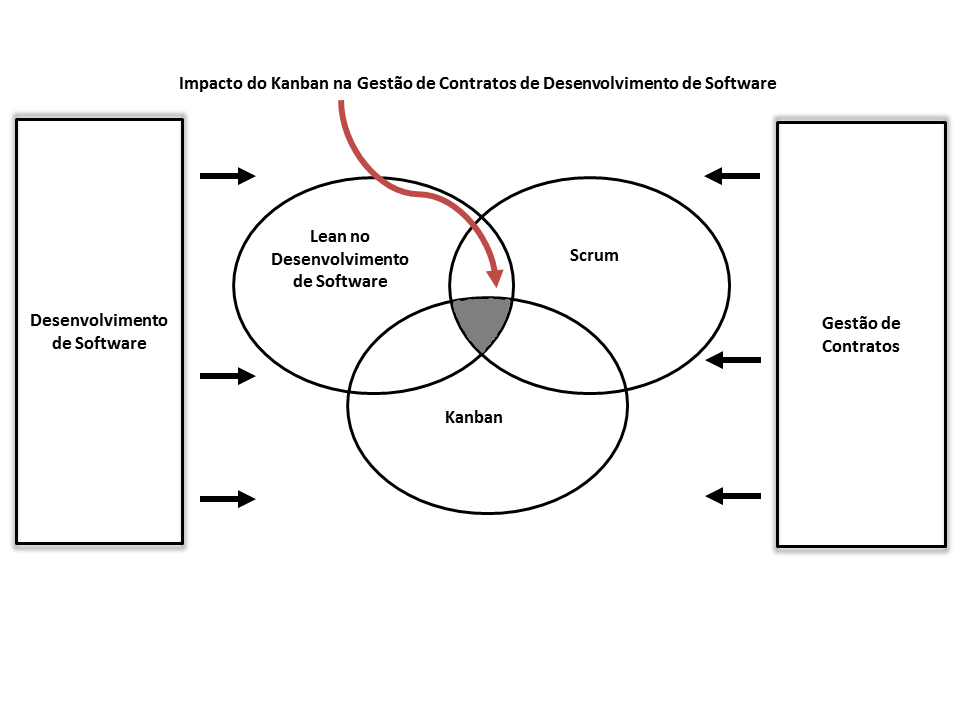
\includegraphics[scale=0.8]{figuras/escopoEC.png}
		\label{escopo}
		\caption{Escopo do Estudo de Caso}
		
\end{figure}

Assim, a proposta deste trabalho consiste na investigação, coleta, análise e discussão dos resultados, de dados de uma contratação de fornecedor de desenvolvimento de \textit{software} pelo Instituto do Patrimônio Histórico e Cultural (IPHAN). A partir da análise  dos dados será realizada uma comparação entre os resultados obtidos com o estudo de caso e os efeitos percebidos pelos principais envolvidos no contrato. O foco será a análise da solução desenvolvida pela organização, a qual é alinhada com os métodos ágeis, com o pensamento lean e com a fase de Gerenciamento do Contrato.


Este trabalho foi estruturado conforme ilustrado na Fig. (14).

\begin{figure}[H]
		\centering
		\label{fig01}
			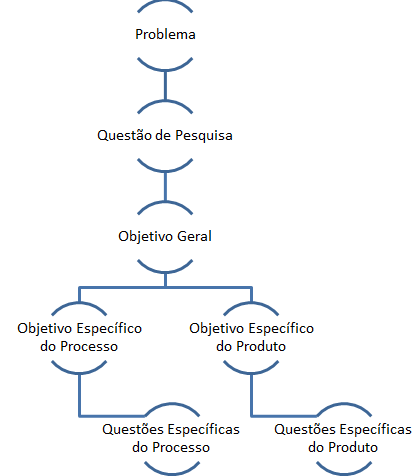
\includegraphics[scale=1.0]{figuras/estruturaEstudo.png}
		\caption{Estrutura do Estudo de Caso}
	\end{figure}

O problema refere-se ao problema de pesquisa identificado. A questão de pesquisa refere-se a questão de pesquisa que foi derivada do problema. Para responder a questão de pesquisa foram construídos dois GQM's (Goal, Question, Metric). Cada GQM possui um objetivo e questões específicas para coleta de métricas a partir de determinada fonte, a fim de atingir o objetivo e responder a questão de pesquisa do trabalho. Ao todo foram definidas onze questões de pesquisa específicas que serão analisadas no estudo de caso. A definição dessa estrutura está a seguir.

\textbf{Problema:} Alguns contratos de desenvolvimento de software da organização não resultaram na entrega do software requisitado ao final do contrato.

\textbf{Questão de Pesquisa:} Como o uso de métodos ágeis e do pensamento lean na gestão de contratos de fornecedores de desenvolvimento de software influenciaram no resultado final do contrato do ponto de vista do gestor de contrato e do fiscal técnico do contrato, que juntos gerenciam o contrato?


\textbf{OE1. Objetivo do Processo:} Analisar a influência do uso de métodos ágeis e do pensamento lean na gestão de contrato do contrato do Sistema Integrado de Conhecimento e Gestão (SICG) com a empresa EGL - Engenharia do ponto de vista do gestor de contrato.

\textbf{Questões Específicas do Processo:}


\textbf{QE1.}  Qual a quantidade total de ordens de serviço?

\textbf{Fonte:} Documentação

\textbf{Métrica:} quantidade total de ordens de serviço.
 
\vspace{\onelineskip} 

\textbf{QE2.} Qual a quantidade de ordens de serviço que tiveram entrega de software funcional?

\textbf{Fonte:} Documentação

\textbf{Métrica:} quantidade de ordens de serviço de software.
 
 \vspace{\onelineskip} 

\textbf{QE3.} Qual a quantidade de ordens de serviço que tiverem entrega apenas de documentação?

\textbf{Fonte:} Documentação

\textbf{Métrica:} quantidade de ordens de serviço de documentação.

 \vspace{\onelineskip} 
 
\textbf{QE4.} Qual a proporção de entrega de software funcional?

\textbf{Fonte:} Documentação

\textbf{Métrica:} quantidade de ordens de serviço de software que tiveram entrega de software funcional /quantidade total de ordens de serviço.

 \vspace{\onelineskip} 

\textbf{QE5.} Qual a duração média de entrega de software funcional?

\textbf{Fonte:}Documentação, scrum master, dono do produto, gestor do contrato, fiscal técnico do contrato, coordenador do projeto.

\textbf{Métrica:} duração total das sprints/duração total das sprints que tiveram de entrega de software funcional.

 \vspace{\onelineskip} 

\textbf{QE6.} Qual a quantidade de ordens de serviço que não teve entrega de software funcional e de documentação?

\textbf{Fonte:} Documentação

\textbf{Métrica:} quantidade de ordens de serviço sem software e documentação.

 \vspace{\onelineskip} 
 
\textbf{QE7.} Qual a porcentagem de requisitos atendidos em cada ordem de serviço?

\textbf{Fonte:} Documentação, dono do produto, gestor do contrato, fiscal técnico do contrato, coordenador do projeto.

\textbf{Métrica:} (requisitos atendidos/requisitos pedidos) * 100.
 
 \vspace{\onelineskip} 

\textbf{QE8.} Quantas multas foram aplicadas no contrato?

\textbf{Fonte:} Documentação, scrum master, dono do produto, gestor do contrato, fiscal técnico do contrato, coordenador do projeto.

\textbf{Métrica}: quantidade de multas.

 \vspace{\onelineskip}  

\textbf{QE9.} Qual o custo de cada sprint do projeto?

\textbf{Fonte:} Documentação

\textbf{Métrica}: custo/sprint.

 \vspace{\onelineskip}  

\textbf{QE10.} O quanto de visibilidade do que estava sendo feito o gestor do contrato teve durante o contrato?

\textbf{Fonte:} Dono do produto, gestor do contrato, fiscal técnico do contrato, coordenador do projeto.

\textbf{Métrica:} alto, médio ou baixo. 
 
 \vspace{\onelineskip} 

\textbf{QE11.} Qual o nível de satisfação com o software entregue ao final do contrato?

\textbf{Fonte:} Dono do produto, gestor do contrato, fiscal técnico do contrato, coordenador do projeto.

\textbf{Métrica:} muito satisfeito, satisfeito, neutro, insatisfeito, muito insatisfeito.
 
 \vspace{\onelineskip} 

\textbf{OE2. Objetivo do Produto:}Analisar a qualidade do código fonte com o uso de métodos ágeis e do pensamento lean na gestão do contrato do contrato do Sistema Integrado 
de Conhecimento e Gestão (SICG) com a empresa EGL - Engenharia do ponto de vista do  e do fiscal técnico do contrato.

\textbf{Questão Específicas do Produto:}

\textbf{QE12.} Qual a qualidade interna do produto entregue até o momento ?

\textbf{Fonte:} Código, scrum master, desenvolvedores, dono do produto, gestor do contrato, fiscal técnico do contrato, coordenador do projeto.

\textbf{Métrica:} bom, excelente, regular e ruim.


\section[Fonte e Método Coleta de Dados]{Fonte e Método de Coleta de Dados}

Os dados foram coletados por meio de entrevistas informais, observações, questionários e por meio da análise de documentos processuais da organização e da base de código fonte de um contrato disponibilizado pelo órgão: o contrato do Sistema Integrado de Conhecimento e Gestão (SICG) com a empresa EGL - Engenharia, no qual foram utilizadas metodologias ágeis para gestão do contrato.Os questionários tinham o objetivo de coletar dados qualitativos e
quantitativos a respeito da organização contratante, do gestor de negócio (cliente) e da empresa contratada no que diz respeito a estrutura organizacional, experiência prévia, satisfação, opniões, percepções e etc. O dados de observação e entrevistas
complementaram os questionários sob o ponto de vista qualitativo.Os dados quantitativos
sobre a execução do processo (solução) e a qualidade do código fonte foram coletados de 20 Sprints do projeto foram coletados da documentação e do código fonte do contrato SICG .

\textbf{Documentos}
\begin{itemize}
\item Processo nº 01450.011592/2010-30, cujo assunto é Contratação de Serviços de Desenvolvimento de Software para o Sistema Integrado de Conhecimento e Gestão (SICG). 
\item Processo vº 01450.000845/2012-10, cujo assunto é Gestão de Contrato IPHAN Nº 28/2011 - Desenvolvimento de Software para o Sistema Integrado de Conhecimento e Gestão (SICG). 
\item Código Fonte do Sistema Integrado de Conhecimento e Gestão (SICG).
\item Backlog do Produto do Sistema Integrado de Conhecimento e Gestão (SICG).
\end{itemize}

\textbf{Questionários}
\begin{itemize}
\item Questionário para os envolvidos no projeto SICG: tem como objetivo coletar informações dos envolvidos no projeto por parte do IPHAN,  fiscal técnico do contrato, coordenador do projeto e do gestor do contrato, que também representa o papel de dono do produto, e dos envolvidos no projeto por parte da empresa contratada, a EGL - Engenharia, scrum master e desenvolvedores.
\end{itemize}

\section[Validade]{Validade}

As principais ameaças aos estudos de caso aplicáveis a este estudo de caso
são mencionadas por Yin (2009). Dentre elas, destaca-se a confiabilidade dos dados
coletados e dos resultados obtidos. Para Seaman (1999), o uso de várias fontes de dados
e métodos de coleta permite a triangulação, uma técnica para confirmar se os resultados
de diversas fontes e de diversos métodos convergem. Dessa forma é possível aumentar a
validade interna do estudo e aumentar a força das conclusões. Nesta pesquisa houve
triangulação de dados  e de metodologia. A triangulação de dados se deu
pelo uso de base de documentos e código organizacionais, questionários e entrevistas para coletar dados. A triangulação
de métodos ocorreu pelo uso de métodos de coleta quantitativos e qualitativos.


\section[Trabalho de Campo]{Trabalho de Campo}

O trabalho de campo é parte fundamental do estudo de caso, por meio dele que os dados para análise serão coletados. Neste trabalho, as entrevistas informais e a triagem dos processos foram realizadas em campo. Os processos disponibilizados pelo orgão eram extensos, mais de quatro mil páginas, por issso a triagem sobre esses processos foi realizada para solicitação de cópias das partes que mais interessavam para o contexto e objetivos de pesquisa desse estudo.